\chapter{Introduzione}\label{introduzione}

La laringoscopia è una procedura medica utilizzata per ispezionare la laringe e per diagnosticare, ed eventualmente curare, i disturbi della laringe e delle corde vocali.

In particolare ci sono due tipi di laringoscopia, quella indiretta e quella diretta. La prima fa uso di un semplice specchio e di una fonte luminosa, la seconda richiede l'uso di un laringoscopio e una anestesia.

Il laringoscopio è uno strumento che grazie a una fibra ottica, una sorgente luminosa e una telecamera permette di osservare nei minimi dettagli la laringe e tutti gli elementi che la costituiscono come la epiglottide e le corde vocali \cite{giorgio_cenni_2008}. In particolare permette di aiutare a diagnosticare malattie come la laryngeal squamous cell carcinoma (SCC), la cui diagnosi precoce riduce la mortalità del paziente \cite{moccia_larynge}.

L'obiettivo di questa tesi è quello di usare algoritmi di apprendimento automatico basati sul transfer learning e sul  preprocessing di immagini  per la classificazione dei frame di una laringoscopia, in particolare ci concentriamo nella la selezione degli informative-frame e lo scarto di tutti i frame non utili: come frame pieni di saliva o non a fuoco. In \cref{fig:larynges} alcuni esempi di frame da selezionare estratti da una laringoscopia.

\begin{figure}[ht]
    \centering
    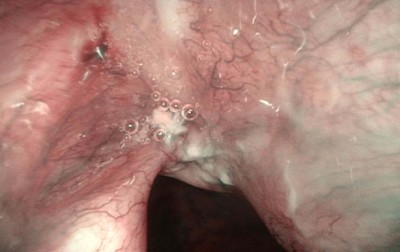
\includegraphics[width=0.3\textwidth]{introduzione/Larynge-1.jpg}
    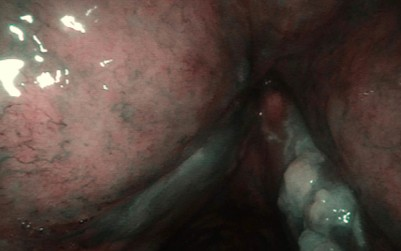
\includegraphics[width=0.3\textwidth]{introduzione/Larynge-2.jpg}

    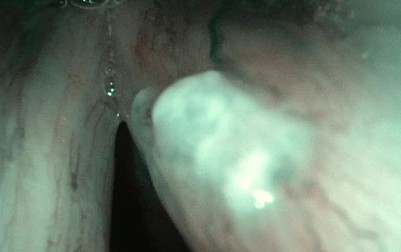
\includegraphics[width=0.3\textwidth]
    {introduzione/Larynge-3.jpg}
    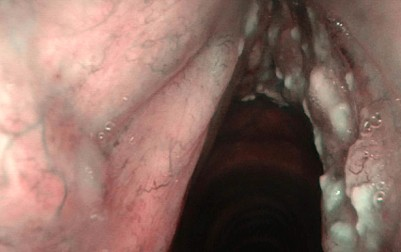
\includegraphics[width=0.3\textwidth]{introduzione/Larynge-4.jpg}
    \caption{Esempio di fotogrammi endoscopici laringei}
    \label{fig:larynges}
\end{figure}

\section{Descrizione dei dataset}\label{descrizione-dei-dataset}

Le prestazioni delle caratteristiche estratte dalla
\gls{cnn} sono state valutate sul dataset
NBI-InfFrames  che
è stato costruito da 18 video endoscopici NBI, riferiti a
18 diversi pazienti affetti da carcinoma a cellule squamose
(SCC). Tutti i video sono stati acquisiti con un sistema endoscopico
NBI (processore video Olympus Visera Elite S190 e
un videoscopio rino-laringo ENF-VH) con frame rate di
25 fps e dimensioni dell'immagine di \(1920\times 1072\) pixel.

Il dataset NBI-InfFrames consiste in un totale di 720 frame, che sono equamente divisi in quattro classi: informative (I), sfuocato (B), con saliva o riflessi speculari (S) e underexposed  (U). 

Per ciascuno dei 18 video endoscopici NBI, i fotogrammi video sono stati estratti a caso e
presentati prima a due valutatori umani. Poi, ai due valutatori è stato chiesto di etichettare i fotogrammi. Nel caso in cui i due
valutatori non fossero d'accordo sulla classe, a un terzo valutatore è stato
chiesto di scegliere la classe definitiva tra le due proposte
dai due valutatori. Questo processo è stato ripetuto fino a quando tutti i
720 fotogrammi sono stati estratti e classificati dai video.

\begin{figure}[ht]
    \centering
    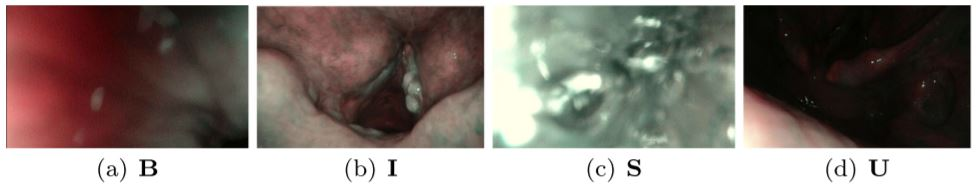
\includegraphics[width=0.9\textwidth]{introduzione/Larynge.jpg}
    \caption[Esempio di fotogrammi endoscopici laringei di NBI-InfFrames]{Esempio di fotogrammi endoscopici laringei di NBI-InfFrames divisi per I: informative, sfuocato: B, S: con
    saliva o riflessi speculari,
    U: underexposed}
    \label{fig:larynges}
\end{figure}

Il secondo dataset è basato sugli informative-frame del dataset precedente, in particolare è stato effettuato un ritaglio delle immagini per mostrare   alcuni dettagli del tessuto umano, il procedimento è mostrato nella \cref{fig:dataset2}. In \cref{fig:dataset2ml} sono mostrati alcuni frame catalogati il dataset 2 è catalogato in base allo stato del tessuto, in particolare Blu: tessuto con intraepithelial papillary capillary loop-like vessels; Giallo: tessuto con Leukoplakia;
Verde: tessuto sano; Rosso: tessuto con hypertrophic vessels \cite{moccia_larynge}.

\begin{figure}[ht]
    \centering
    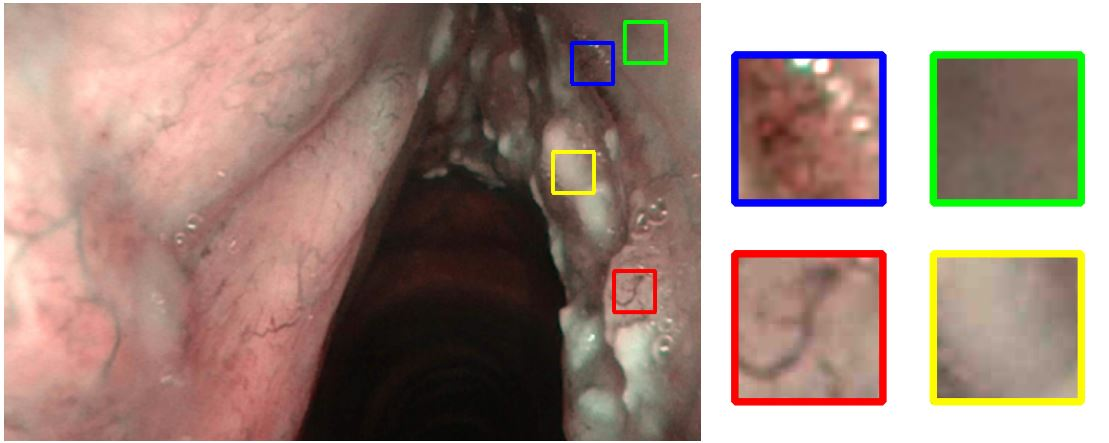
\includegraphics[width=0.9\textwidth]{introduzione/dataset-2.JPG}
    \caption{Esempio di come sono state estratte le immagini del dataset 2}
    \label{fig:dataset2}
\end{figure}

\begin{figure}[ht]
    \centering
    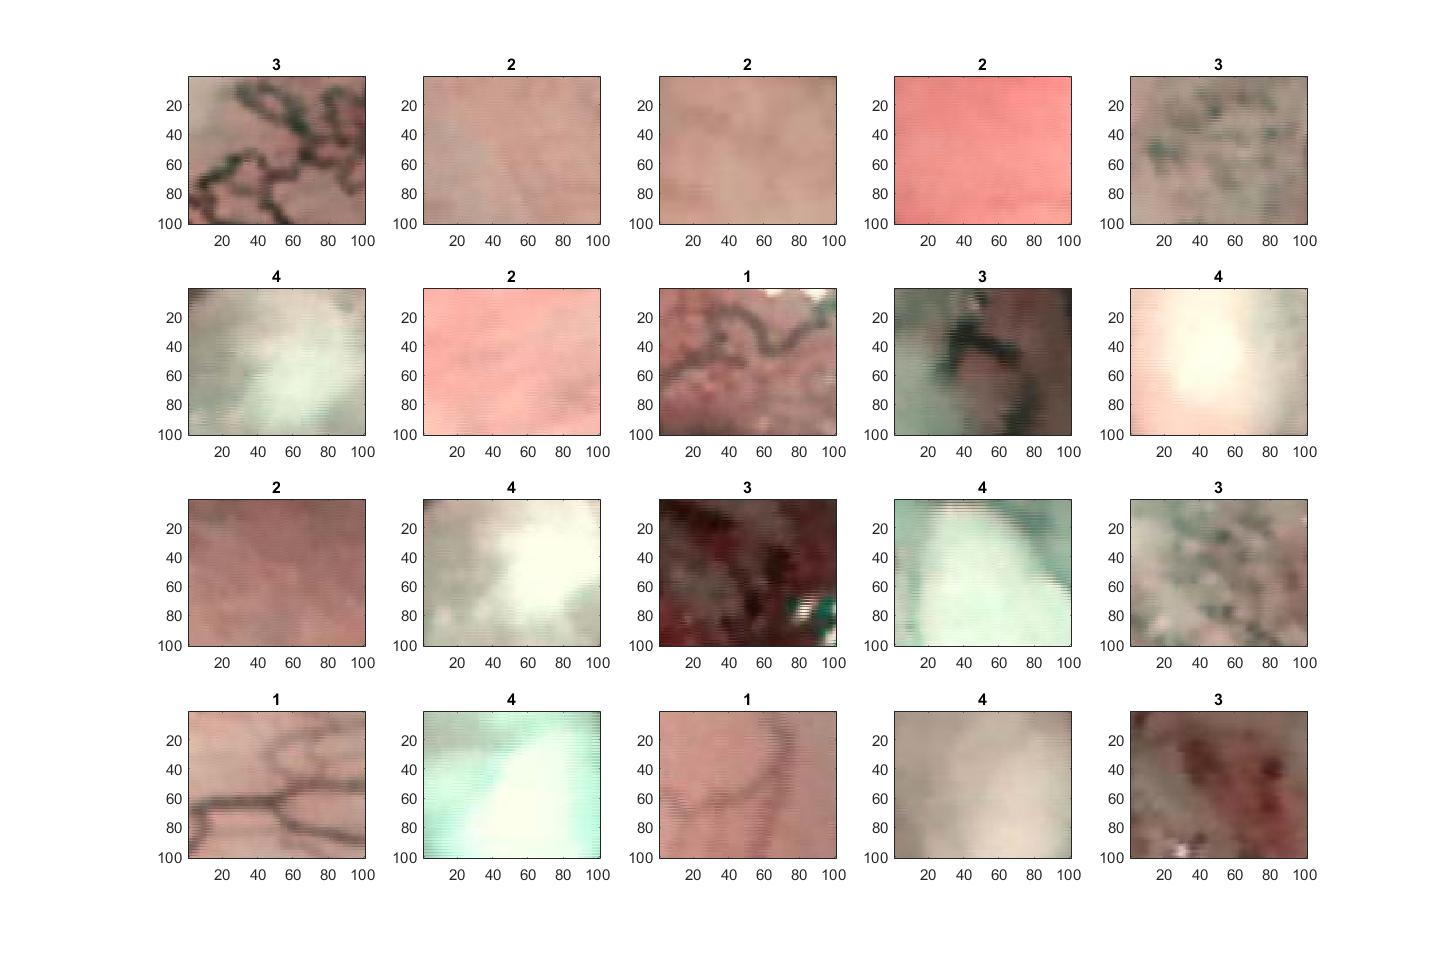
\includegraphics[width=0.9\textwidth]{introduzione/dataset-2-ml.JPG}
    \caption[Esempio di immagini del dataset 2]{Esempio di immagini del dataset 2, le varie classi sono suddivise in base allo stato del tessuto in relazione alla SCC.}
    \label{fig:dataset2ml}
\end{figure}

\section{Lavori precedenti}\label{lavori-precedenti}